%	Dependencies: texlive texlive-lang-german texlive-latex-recommended texlive-xetex cm-super kile biber 
%
%
%	main.tex
%
%	main for Master Thesis @ QW TU Berlin 
%
%	author: Rudolph R. Maier	
%
%	TU Berlin - 2018
%
%	Zur Benutzung von Bibtex und Biblatex: http://www.ub.uni-konstanz.de/serviceangebote/literaturverwaltung/bibtex/bibtex-und-biblatex-benutzen.html
%				Bibtex:		\renewcommand{\bibname}{Literaturverzeichnis} 
%
%	für Biber: tex.stackexchange.com/questions/26516/how-to-use-biber
% 		   pdflatex biber pdflatex
%
%% 	definiert Dokumenttyp und Grundlegende Einstellungen:
%
%
\documentclass[a4paper,oneside,11pt,titlepage,	%, captions=nooneline	% captions=nooneline --> flushleft
% twocolumn
% bibtotoc, liststotoc, % obsolete options 
% longbibliography % deprecated: bibtex option
% bibtotoc - Lit.VZ im Inha1ltsVZ
]{scrreprt}
				
\usepackage[
% 	colorlinks=true,
% 	urlcolor=blue,
% 	linkcolor=red,
	pdfauthor={Rudolph Ribeiro Maier},
	pdftitle={Titel der Masterarbeit},
% 	pdfsubject={The Subject},
% 	pdfkeywords={Some Keywords},
	pdfproducer={Latex with hyperref},
 	pdfcreator={pdflatex}
	bookmarks,				% PDF index
]{hyperref}
						%	KOMA Script (als Europäische  Anpassung vorzuziehen) 
% 						%	scrartcl, scrreprt, scrbook, scrlttr2

%% Codierung
\usepackage[utf8]{inputenc}			%	Codierung im Editor fuer direkte Eingabe der Sonderzeichen (WIN: latin1 oder ansinew, MAC: applemac, alt.: utf8)
\usepackage[T1]{fontenc}			%	U.A. damit Umlaute in PDF Dokumenten gefunden werden,  (T1: PostScript Type 1)
\usepackage[ngerman]{babel}			%	Anpassung der Überschriften und Silbentrennung (ngerman. english,...)
%		
%% Seitenränder
% 
\usepackage{geometry}
\geometry{left=30mm, right=30mm, top=20mm, bottom=20mm}
% Disable single lines at the start of a paragraph (Schusterjungen)
\clubpenalty = 10000
% Disable single lines at the end of a paragraph (Hurenkinder)
\widowpenalty = 10000
\displaywidowpenalty = 10000

%    Kein Einrücken der Absätze
\setlength{\parindent}{0pt}

% Zeilenabstand & Font
\usepackage[doublespacing]{setspace}			% singlespacing, onehalfspacing, doublespacing
							% wird später für den Fließtext mit \linespread{x} definiert

% % % % % % % % % % % % % % % % % % % % % % % % % % % % % % % % % % % % % % % % % % % % % % % % % % % % % % % 
% 
%	FONT SELECTION with Math support from The LATEX Font Catalogue: www.tug.dk/FontCatalogue
% 	Test with pdffonts main.pdf
% 
% \newcommand{\changefont}[3]{
% \fontfamily{#1} \fontseries{#2} \fontshape{#3} \selectfont}
% \renewcommand{\rmdefault}{lmr}
% 
% \addtokomafont{sectioning}{\rmfamily} 		% 	Überschriften mit Serifen!
% 
% 	Latin Modern - Enhanced Computer Modern
% 
% \usepackage{lmodern}	% works: LMRoman12-Regular
% 
%
% 	EB Garamond (T1)	The default is oldstyle numbers. I have set the numbers to be lining to display lining numbers as well as oldstyle numbers
% 
% \usepackage[lining,scaled=.95]{ebgaramond} % works: EBGaramond12-Regular 		
% 
% 
% 	Garamond
% 
% \usepackage[urw-garamond]{mathdesign}	% works: GaramondNo8-Reg	 (~/texmf/fonts/type1/...)
% 
% 
% 	Nimbus Roman, is a clone of Times
% 
% \usepackage{nimbus} % ?? SFRM1200
% 
% 
% 	TIMES
% 
% \usepackage{mathptmx}	% works: NimbusRomNo9L-Regu - das hatte ich in der BA für den Fließtext
% 
% 
% 	TEX Gyre Termes, an Enhanced Time font
% 
% \usepackage{tgtermes} %	works: TeXGyreTermes-Regular 
% 
% 
% 	Palatino
% 
% \usepackage[sc]{mathpazo} % works: URWPalladioL-Roma
% \linespread{1.05}         % Palatino needs more leading (space between lines)
% 
% 
% 	KP Serif
% 
% \usepackage{kpfonts} % works: Kp-Regular
% 
% 
% 	Utopia Regular with Fourier, nur eine von beiden verwenden
% 
% \usepackage{fourier} % works: Utopia-Regular
% \usepackage[adobe-utopia]{mathdesign} % works: Utopia-Regular
% 
% 	
% 	Helvetica SANS SERIF
% 
\usepackage[scaled=0.9]{helvet}
% 
% 

\renewcommand*{\rmdefault}{\sfdefault}			% definiert serifenlos für serifenschrift (Grundtext). http://texwelt.de/wissen/fragen/785/wie-stelle-ich-alle-schrift-in-meinem-dokument-auf-serifenlos


% New header
\usepackage{fancyhdr}
\fancypagestyle{text}{%
  % flush all default styles
  \fancyhf{} 
  % Left part of the Header
  \fancyhead[LO]{\nouppercase{\leftmark}}
  % Center Part of the header
  \fancyhead[C]{}
  % Right part of the header
  \fancyhead[RO]{\thepage}
  % upper ruler
  \renewcommand{\headrulewidth}{0.4pt}
}
\fancypagestyle{plain}{%
  % flush all default styles
  \fancyhf{} 
  % Left part of the Header
  \fancyhead[LO]{\nouppercase{\leftmark}}
  % Center Part of the header
  \fancyhead[C]{}
  % Right part of the header
  \fancyhead[RO]{\thepage}
  % upper ruler
  \renewcommand{\headrulewidth}{0.4pt}
}
\fancypagestyle{fzvz}{%
  % flush all default styles
  \fancyhf{} 
  % Left part of the Header
  \fancyhead[LO]{\nouppercase{\leftmark}}
%   \fancyhead[LO]{FOOOO}
  % Center Part of the header
  \fancyhead[C]{}
  % Right part of the header
  \fancyhead[RO]{\thepage}
  % upper ruler
  \renewcommand{\headrulewidth}{0.4pt}
%   \renewcommand{\chaptermark}[1]{\markboth{#1}{}}
}


% 
%% Mathematik
\usepackage{amssymb}				%	Mathematische Symbole (Pfeile etc...)
\usepackage{amsfonts}
\usepackage{amsmath}				%	Fuer Mathematische Gleichungen

\usepackage[right]{eurosym}			% 	Eurozeichen 
\usepackage{amsopn}				%	für \grad
\DeclareMathOperator{\grad}{grad}		%	für \grad

% 
%Setzt den equation-Zaehler nach jeder Section zurueck
% \numberwithin{equation}{section}	
%
%% Content Management
\usepackage{subfigure} 				%	Grafiken nebeneinander : http://www.golatex.de/zwei-bilder-nebeneinander-t1915.html
\renewcommand{\floatpagefraction}{.8}		% 	Figure Objekte erst ab x % alleine auf einer Seite ohne Text
% \begin{figure} 
%     \subfigure[Bezeichnung der linken Grafik]{\includegraphics[width=0.49\textwidth]{ordner/name1.jpg}} 
%     \subfigure[Bezeichnung der rechten Grafik]{\includegraphics[width=0.49\textwidth]{ordner/name2.jpg}} 
% \caption{Titel unterm gesamten Bild} 
% \end{figure}
\usepackage{pstricks}				% 	PSTRICKS .tex Grafiken von DIA 
\usepackage{tikz}				% 	einbinden von DIA Grafiken (PGF?)
\usepackage{graphicx}				%	einbinden von Graphiken :	\includegraphics{schachbrett.eps}
\usepackage{colortbl}				% 	Für \rowcolor[gray]{0.9} zum Einfärben von Tabellenzeilen
% \graphicspath{{img/}}
% 
\usepackage{pdfpages} 				%	PDF include : 			\includepdf[pages={5,8,10-14}]{internal_rate_of_return.pdf}
\usepackage{listings}				%	Wie \begin{verbatim} : 		\begin{lstlisting}
						%	add hypertext capabilities
% 
% disable fucking ugly boxes
\hypersetup{pdfborder = 0 0 0}
% \booktabs					%	Für die Tabellen
\usepackage{tabularx}
%\usepackage{pdflscape}				%	Querformat
%\usepackage{enumitem}				%	Für bessere nummerierungen
%
% VON MAX
%\usepackage{subfigure}                         % mehrere Graphiken in einer Abbildung
%\usepackage{float}                             % erweiterte floating Befehle
%\usepackage[section]{placeins}                 % definiert \FloatBarrier
\usepackage[locale=DE]{siunitx}	
% 
% 
\usepackage[
    backend=biber,
    style=alphabetic, 	%numeric,
    bibstyle=alphabetic,
    sortlocale=de_DE,
%     natbib=true,
%     url=false, 
    isbn=false,
    doi=true,
%     defernumbers=true, % 
%     ibidtracker=context, %damit ebd. funktioniert 
%     eprint=false
]{biblatex} % Biber 
\usepackage{csquotes}				% When using babel or polyglossia with biblatex, loading csquotes is recommended to ensure that quoted texts are typeset according to the rules of your main language.
\addbibresource{../10_research/bibliography/main.bib}
% 	Name, Vorname: 
\DeclareNameAlias{default}{last-first}
%	Doppelpunkt nach Autor ( Anstatt Punkt)
\renewcommand*{\labelnamepunct}{\addcolon\addspace}
%
% \usepackage{german,longtable}
%

%------------------------------------------------------
% Add Glossary Functionality
\usepackage[
nonumberlist, 	% don't display page location where Term is used
acronym,      % create acronym list
% toc,           % Add GLossary location to Table of Contents..
% section
]      % ..as a section/chapter (but without number!)
{glossaries}
%
% Make \gls not fragile (useful if used within \caption{})
\robustify{\gls}
\robustify{\glspl}
%
% deactivate the default . after descriptions in the Glossary
\renewcommand*{\glspostdescription}{}
 
% Let the makefile build a glossary
\makeglossaries
%
% Include glossary.tex file with all the definitions
% usage: \gls{id}
%
\newglossaryentry{xxx}
{
  name=xx, 
  description={xxx}
}
%
%
\newglossaryentry{jit}
{
  name=Just-in-time, 
  description={Just-in-time-Produktion oder auch bedarfssynchrone Produktion}
}
%
%
\newglossaryentry{bmc}
{
  name=BMC, 
  description={Business Model Canvas}
}
%
%
\newglossaryentry{ishikawa}
{
  name=Ishikawa, 
  description={Ursache-Wirkungs-Diagramm}
}
%
%
\newglossaryentry{fta}
{
  name=FTA, 
  description={Fault Tree Analysis}
}
%
%
\newglossaryentry{plz}
{
  name=PLZ, 
  description={Produktlebenszyklus}
}
%
%
\newglossaryentry{pdm}
{
  name=PDM, 
  description={Produktdatenmanagement}
}
%
%
\newglossaryentry{dsm}
{
  name=DSM, 
  description={Design Structure Matrix, Methode zur Analyse von hochvernetzten Systemen}
}
%
%
\newglossaryentry{atlas}
{
  name=Atlas.ti, 
  description={Software zur qualitativen Datenanalyse}
}
%
%
\newglossaryentry{kvp}
{
  name=KVP, 
  description={Kontinuierlicher Verbesserungsprozess}
}
%
%
\newglossaryentry{pdca}
{
  name=PDCA, 
  description={Plan, Do, Check, Act}
}
%
%
\newglossaryentry{fmea}
{
  name=FMEA, 
  description={Failure Mode and Effects Analysis}%. Ein QM-Werkzeug für die systematische Bewertung von Risikofolgen.}
}
%
%
\newglossaryentry{qfd}
{
  name=QFD, 
  description={Quality Function Deployment}%. Methode zur Analyse und Darstellung von mehrdimensionalen Korrelationen}
}
%
%
\newglossaryentry{pep}
{
  name=PEP, 
  description={Produktentstehungsprozess}
}
%
%
\newglossaryentry{gps}
{
  name=GPS, 
  description={Ganzheitliche Produktionssysteme nach VDI 2870}
}
%
%
\newglossaryentry{kmu}
{
  name=KMU, 
  description={Kleine und mittelständische Unternehmen}
}
%
%
\newglossaryentry{obeya}
{
  name=Obeya, 
  description={Vereinigung aller beteiligten Personen bei der Entwicklung in einem großen Raum (Teil des Toyota Produktionssystems)}
}
%
\newglossaryentry{iot}
{
  name=IoT, 
  description={Internet of Things}
}
%
%
\newglossaryentry{erp}
{
  name=ERP, 
  description={Enterprise Resource Planning}
}
%
\newglossaryentry{ipdm}
{
  name=IPDM, 
  description={Integrierte Produktdatenmodelle}
}
%
\newglossaryentry{lsu}
{
  name=LSU, 
  description={Lean Start-up}
}
\newglossaryentry{sop}
%
{
  name=SOP, 
  description={Beginn der Serienproduktion}
}
%
\newglossaryentry{smed}
{
  name=SMED, 
  description={Single Minute Exchange of Dies}%, Methode zur Senkung von Rüstzeiten}
}
%
\newglossaryentry{heijunka}
{
  name=Heijunka, 
  description={
%(平準化),
Harmonisierung des Produktionsflusses}
}

\newglossaryentry{bspw}
{
  name=bspw.,
  description={Beispielsweise}
}
%
\newglossaryentry{mvp}
{  
  name=MVP,
  description={Minimal überlebensfähiges Produkt, engl.: Minimum Viable
Product}
}

%
%%====================================================================================================
%
%
%------------------------------------------------------
% Add Blank page Functionality
\usepackage{afterpage}
\newcommand\blankpage{%
    \null
    \thispagestyle{empty}%
    \addtocounter{page}{-1}%
    \newpage}
%     
%%====================================================================================================


% % % % % % % % % % % % % % % % % % % % % % % % % % % % % % % % % % % % % % % % % % % % % % % % % % % % % % % 
\begin{document}
%
% \changefont{ptm}{m}{n}
% 
\setcounter{page}{-1}
\pagenumbering{roman}
% % \includepdf{./img/deckblatt.pdf}
% 
% \titlehead
% {Technische Universität Berlin\\
% Fakultät V  Verkehrs- und Maschinensysteme\\
% Institut für Werkzeugmaschinen und Fabrikbetrieb IWF\\
% Fachgebiet Qualitätswissenschaft\\
% Prof. Dr.-Ing. Roland Jochem\\
% Dipl.-Ing. Robert Mies
% \\
% }
% 
% \subject{Masterarbeit}
% % 						%
% \title{Entwicklung eines Anlaufmodells für das Lean Start-up}
% % 						%
% \subtitle{\author{Rudolph Ribeiro Maier (330466)} 
% }
% 						
% \date{19.07.2018}
% 
% \maketitle

\begin{titlepage}
\begin{flushright}
\includegraphics[scale=0.4]{./img/tu-logo-eps-converted-to.pdf}\\[2.5cm] % Include a department/university logo - this will require the graphicx package
\end{flushright}

\newcommand{\HRule}{\rule{\linewidth}{0.5mm}} % Defines a new command for the horizontal lines, change thickness here

\center % Center everything on the page
 
%----------------------------------------------------------------------------------------
%	HEADING SECTIONS
%----------------------------------------------------------------------------------------

\textsc{\LARGE Masterarbeit}\\[1.5cm] % Name of your university/college
\textsc{\Large Technische Universität Berlin\\Fakultät V  Verkehrs- und Maschinensysteme}\\[0.5cm] % Major heading such as course name
\textsc{\large Institut für Werkzeugmaschinen und Fabrikbetrieb IWF\\Fachgebiet Qualitätswissenschaft\\Prof. Dr.-Ing. Roland Jochem}\\[2.5cm] % Minor heading such as course title

%----------------------------------------------------------------------------------------
%	TITLE SECTION
%----------------------------------------------------------------------------------------

\HRule \\[0.6cm]
{ \huge \bfseries Entwicklung eines Anlaufmodells \\für das Lean Start-up}\\[0.4cm] % Title of your document
\HRule \\[3cm]
 
%----------------------------------------------------------------------------------------
%	AUTHOR SECTION
%----------------------------------------------------------------------------------------
% \begin{flushleft}
\begin{tabular}{ll}
Verfasser: & Rudolph Manuel \textsc{Ribeiro Maier} \\
Studiengang: & Maschinenbau \\
% Matr.-Nr.: & 330 466 \\
E-Mail: & rudolph@ribeiromaier.de \\[1cm]
Betreuer: & Prof. Dr.-Ing. Roland \textsc{Jochem} \\
& Dipl.-Ing. Robert \textsc{Mies}
\end{tabular}\\[2cm]
 
% \end{flushleft}

 

% \begin{minipage}{0.4\textwidth}
% \begin{flushleft} \large
% \emph{Autor:} Rudolph Manuel \textsc{Ribeiro Maier} \\% Your name
% \emph{Martikel-Nr.:} 330466
% \end{flushleft}
% \end{minipage}
% ~
% \begin{minipage}{0.4\textwidth}
% \begin{flushright} \large
% \emph{Betreuer:} \\
% Prof. Dr.-Ing. Roland \textsc{Jochem}\\ % Supervisor's Name
% Dipl.-Ing. Robert \textit{Mies}
% \end{flushright}
% \end{minipage}\\


% If you don't want a supervisor, uncomment the two lines below and remove the section above
%\Large \emph{Author:}\\
%John \textsc{Smith}\\[3cm] % Your name

%----------------------------------------------------------------------------------------
%	DATE SECTION
%----------------------------------------------------------------------------------------

{\large Berlin, 19. Juli 2018}\\[2cm] % Date, change the \today to a set date if you want to be precise

%----------------------------------------------------------------------------------------
%	LOGO SECTION
%----------------------------------------------------------------------------------------

% \includepdf[scale=0.2]{./img/tu-logo-eps-converted-to.pdf}
 
%----------------------------------------------------------------------------------------

\vfill % Fill the rest of the page with whitespace

\end{titlepage}


  
  % Titelblatt der Arbeit
%   \begin{titlepage}
% 
%   \includepdf[scale=0.2]{./img/tu-logo-eps-converted-to.pdf}
% %     \includegraphics[scale=0.45]{./img/tu-logo-eps-converted-to.pdf }
%     \vspace*{2cm} 
% 
%  \begin{center} \large 
%     
%     Masterarbeit
%     \vspace*{2cm}
% 
%     {\huge Titel der Bachelorarbeit}
%     \vspace*{2.5cm}
% 
%     Name des Autors
%     \vspace*{1.5cm}
% 
%     Datum der Abgabe
%     \vspace*{4.5cm}
% 
% 
%     Betreuung: Name der Betreuerin / des Betreuers \\[1cm]
%     Fakult\"at für Mathematik \\[1cm]
% 		Karlsruher Institut für Technologie
%   \end{center}
% \end{titlepage} % This is the titlepage
\maketitle
% \includepdf{latex_settings/AUF1_70.pdf}			% Aufgabenstellung
% \includepdf{latex_settings/AUF2_70.pdf}
% \blankpage
%
%
%=====================================================
% Load Declaration of Authorship
\newpage
\pagestyle{text}
\thispagestyle{empty}
\section*{Eidesstattliche Erklärung}
\begin{verbatim}

\end{verbatim}
Hiermit erkl\"{a}re ich, % Rudolph Manuel Ribeiro Maier, 
dass ich die vorliegende Arbeit %, betitelt  \textit{\enquote{Design eines Energie Harvesting Moduls für autonome Energieversorgung von Bodensensoren}} 
selbstst\"{a}ndig und eigenh\"{a}ndig sowie ohne unerlaubte fremde Hilfe und ausschließlich unter Verwendung der aufgef\"{u}hrten Quellen und Hilfsmittel angefertigt habe. \\

Die selbstständige und eigenständige Anfertigung versichert an Eides statt:

\begin{verbatim}

\end{verbatim}
\hrulefill\\
\hspace*{2cm}Unterschrift
\hfill
Berlin, 19. Juli 2018

%=====================================================
%
% \include{acknowledgment}
% \include{summary}
% \newpage
% 
% \begin{abstract}
\chapter*{Zusammenfassung}
% %  Ziele / Problemstellung
% Steigende Innovationszyklen, kürzere Produktlebenszyklen und eine höhere Variantenvielfalt bilden heute die größten Herausforderungen für die produzierende Industrie. Somit bekommen Serienanläufe einen wachsenden Einfluss auf den wirtschaftlichen Erfolg des Produkts. 
% Durch die kontinuierlich sinkende Wertschöpfungstiefe setzt sich der Gesamtanlauf aus vielen Einzelanläufen zusammen. Dadurch erhöht sich die Komplexität des Gesamtanlaufs. 
Serienanläufe stellen aufgrund ihrer zunehmenden Komplexität immer größere Herausforderungen an produzierende Unternehmen. Dies gilt insbesondere für Lean Start-ups (\gls{lsu}), die oft nicht über ein systematisches Anlaufmanagement verfügen.
Gegenstand dieser Arbeit ist die Entwicklung eines Leitfadens zur optimalen Umsetzung einer Best-Practice für den Serienanlauf im \gls{lsu}.

% % Lösung: 
% GG
Da bisher in der Literatur keine einheitliche Auffassung über Anlaufmanagement im Allgemeinen herrscht, wurden zunächst fünf wichtige Quellen identifiziert. Mit Hilfe des Tools \textit{\gls{atlas}} wurden die Themenkomplexe strukturiert und konsolidiert in einem Grundgerüst abgebildet. Dieses setzt sich aus strategisch konzeptionellen und operativen Aspekten zusammen und bildet die Struktur für die weitere Arbeit. 
%  Literaturrecherche
Anhand des Grundgerüsts erfolgte eine Literaturrecherche, die den Stand der Wissenschaft bzgl. der Themenkomplexe abbildet. Es wurden geeignete Methoden und Gestaltungsempfehlungen identifiziert und in den Kontext eingeordnet. 
% Leitfaden
Schließlich wurde ein Leitfaden nach Vorbild des Business Model Canvas erstellt. Dieses soll einem Unternehmer anhand von spezifisch zu beantwortenden Fragen helfen, zielgerichtet fundierte Entscheidungen hinsichtlich der Gestaltung eines Serienanlaufs zu treffen. 
% 

% % Impact
% Wissenschaft
Das hier entwickelte Grundgerüst sowie der Leitfaden können als Grundlage für weitere Forschung dienen. Diese kann sowohl hinsichtlich Quantität (\gls{bspw} weitere Literaturrecherche) als auch hinsichtlich Qualität (Erweiterung des Grundgerüsts) variiert werden. Denkbar ist auch eine Änderung der Betrachtungsebene. Für die wissenschaftliche Validierung der Erkenntnisse bietet sich empirische Forschung oder Ac­tion-Re­search an. 
% Bemerkung zu allg. Handlungsempfehlungen. Ggf. zu viel für das Abstract??
Weiterhin ist zu beachten, dass der Leitfaden lediglich zu gestaltende Aspekte abbildet. Im Hauptteil sind jedoch viele allgemeine Handlungsempfehlungen identifiziert worden, welche im Leitfaden nicht darstellbar sind. Diese sind jedoch von großem Interesse uns sollten \gls{bspw} in einem \textit{Handbuch Anlaufmanagement für das \gls{lsu}} zusammengefasst werden.
% 
% Wirtschaft
In der Praxis ermöglicht der Leitfaden kaufmännisch geprägten Gründern fundierte Entscheidungen zu treffen. Voraussetzungen dafür sind eine hohe Motivation sowie vorhandene Ressourcen. Ebenfalls ist ein Verständnis der Grundbegriffe aus Produktion und Qualitätsmanagement erforderlich. 
%  2061 characters

\chapter*{Abstract}
Manufacturing ramp-ups challenge the manufacturing industry due to growing complexity. This affects especially the Lean Startup (\gls{lsu}), since it doesn't have a systematically set up ramp-up management. The purpose of this Thesis is to develop a guideline which supports the setup of a proper ramp-up management in \gls{lsu}s. 

Since there is no uniform interpretation of ramp-up management in literature, five relevant sources were identified. Supported with the tool \textit{\gls{atlas}}, these five interpretations were structured and unified into a basic framework. It consists of strategic-conceptual and operational elements and provides the structure for the further work of the thesis. The literature research was based on this framework, and represents the current state of science and technology. Suitable methods and design recommendations were identified and put in context. Finally, the results were formulated into a guideline, which follows the design of the \textit{Business Model Canvas}. This guideline contains specific questions, which lead to profound decisions regarding the design of the ramp-up, when answered by the entrepreneur. 

Both the developed framework and the guideline may also provide a frame for further research. % As well...as
The research may be continued in quantitative (e.g. further research depth) as well as qualitative (expanding the framework) aspects. Additionally, the level of abstraction may be changed. Both empirical research and action research are applicable for validation of the results proposed in this Thesis. 
On the other hand, the guideline allows commercial oriented entrepreneurs to take profound decisions in their industial practice. A high level of motivation and available ressources are requirements that need to be met. In addition, the entrepreneur needs to have a basic knowledge of quality management and manufacturing terms. 

% 1870 characters
\addcontentsline{toc}{chapter}{Kurzzusammenfassung}
% \end{abstract}

\tableofcontents
%
% %=====================================================
% Print Glossary
\newpage
% \pagestyle{glossary}
% \glsaddall
\printglossary[%style=altlist,
title=Abkürzungsverzeichnis]%,toctitle=Abkürzungsverzeichnis]
%  Damit erscheint es im InhaltsVZ als chapter. Die eingebaute Funktion beim Laden von glossaries unterstützt nur section, nicht chapter
\addcontentsline{toc}{chapter}{Abkürzungsverzeichnis}
% %
% %=====================================================
% \pagestyle{fzvz}
% % \renewcommand{\chaptermark}[1]{\markboth{#1}{}}
% \newpage
% \chaptermark{Verzeichnis der Formelzeichen}	% für chaptername im fancyheader, nur hier nötig
% \addcontentsline{toc}{chapter}{Verzeichnis der Formelzeichen}
% \input{./tab/fvz1}
% \newpage
% \input{./tab/fvzg1}
% \newpage
% % \addcontentsline{toc}{chapter}{\listfigurename}
% \listoffigures
% \newpage
% \listoftables
% 
%%====================================================================================================
%             				 TEXTANFANG
%%====================================================================================================
%
% \linespread{}

\pagestyle{text}
% Add Left Header
% \onehalfspacing
%
%
% \include{0_work}
\newpage
\setcounter{page}{0}
\pagenumbering{arabic}
% \section{Einführung}
\chapter{Einführung}
\section{Motivation \& Problemstellung}
Die produzierende Industrie findet sich heutzutage in einem zunehmend dynamischen Wettbewerbsumfeld wieder, welches vielschichtige Herausforderungen mit sich bringt \cite{Renner2012}. Die hauptsächlichen Herausforderungen liegen in steigenden Innovationsgeschwindigkeiten, kürzeren Produktlebenszyklen und einer höheren Variantenvielfalt \cite{Kuhn2002,Stauder2016}. Um dem durch die Globalisierung verstärkten Wettbewerb standzuhalten, müssen produzierende Unternehmen innovative Produkte und Dienstleistungen anbieten und sich zunehmend kundenorientiert aufstellen \cite{Surbier2014}. 
Eine zentrale Rolle wird hier dem Anlauf von Serienprodukten zugeschrieben. Aufgrund immer kürzer werdender Produktlebenszyklen rücken Kosten und Zeitaufwand in den Vordergrund \cite{Winkler2007}. So hat der Anlauf einen signifikanten Einfluss auf den wirtschaftlichen Erfolg des Produkts und die Time-to-Volume \cite{Klocke16}. Selbst ein um wenige Monate verschobener Verkaufsstart kann über Erfolg oder Misserfolg des Produkts entscheidend sein \cite{Schuh2008a}. Die Bedeutung der Serienanläufe findet bisher in der Wissenschaft keine angemessene Aufarbeitung \cite{Dyckhoff2012}. 

\section{Fokus der Arbeit}
Der Trend zur Konzentration auf Kernkompetenzen sorgt dafür, dass in großen Unternehmen immer mehr Wertschöpfungsanteile an Zulieferer abgegeben werden  \cite{Hilmola2015, Wildemann2008}. Der Gesamtanlauf setzt sich fortan aus vielen lokalen Einzelanläufen zusammen \cite{Zimolong2006}. Daraus resultieren höhere Abhängigkeiten zwischen größeren Unternehmen und den Zulieferern, die meist mittelständische Unternehmen sind. 

Die Abschlussarbeit soll sich im Speziellen mit dem Serienanlauf im KMU und SME als Zulieferer für größere Unternehmen beschäftigen, da hier erhebliches Verbesserungspotential erkennbar ist \cite[S.18]{Dombrowski2009a}. So gibt es in KMU meist keine Anlaufprozesse. Da es in KMU oft keine Stabsstellen gibt, werden Anläufe von den Mitarbeitern oft zusätzlich zum Tagesgeschäft gesteuert \cite{Dombrowski2009}. %TODO kein Zugriff auf Primärquelle D.Spath!! 
Mangelnde finanzielle und zeitliche Kapazitäten sowie fehlendes Know-how verhindern eine nachvollziehbare Dokumentation sowie proaktive Maßnahmen \cite{Zimolong2006,Dombrowski2009a}. 

Weiterhin soll untersucht werden, wie der Auftraggeber den Anlaufprozess des Lieferanten unterstützen kann. Größere Unternehmen verfügen in der Regel über mehr Ressourcen und teilweise eigene Anlaufprozesse. Im Zuge der Verlagerung der Wertschöpfungsanteile, gewinnt die Innovationskraft von Modul- und Systemlieferanten zunehmend an Bedeutung für den Erfolg eines Produktes \cite{Kuhn2002}. Ein erfolgreiches und effizientes Anlaufmanagement in KMU ist im Sinne der Entwicklung einer nachhaltigen Partnerschaft für Auftraggeber und Lieferant von großer Bedeutung. \textit{Wildemann} erkennt hier das Potenzial von Einspareffekten sowie Nutzung erheblicher Wettbewerbsvorteile auf beiden Seiten \cite{Wildemann2008}.

\textit{Dyckhoff} und \textit{Scholz} sind zu der Erkenntniss gekommen, dass das Thema weder in Industrie noch in der Wissenschaft hinreichend Beachtung findet \cite{Dyckhoff2012, Scholz2010}, weshalb hier keine zufriedenstellenden Ergebnisse zu erwarten sind.
Ziel der Arbeit ist, einen Überblick über den Stand der Forschung zu geben und einen Entwurf für ein Anlaufmodell zu entwickeln. 

\section{Herangehensweise}
Die Abschlussarbeit wird eine Literaturarbeit. In der Einführung erfolgt eine knappe Darstellung der zu behandelnden Themen Lean Startup / KMU und Anlaufmanagement. Im Hauptteil wird zunächst der Stand der Wissenschaft zum Thema Lean Startup skizziert. Den größeren Teil bildet eine umfassende Literaturanalyse zum Stand der Wissenschaft des Anlaufmanagements. Die Literaturrecherche erfolgt nach fest definierten Kriterien. Für die Literaturanalyse werden mit Hilfe des Tools \textit{Atlas.ti} alle relevanten Textstellen gecoded, d.h. identifiziert und nachvollziehbar dokumentiert. Anhand der  Ergebnisse wird anhand von möglichst vielen Quellen der Stand der Wissenschaft dargestellt. Im nächsten Abschnitt werden für das Lean Startup nicht berücksichtigte Anforderungen an das Anlaufmanagement ermittelt und daraus eine Art Anlaufmodell abgeleitet. 

Die Validierung der Ergebnisse erfolgt durch Zitierung der Quellen. Auf eine Validierung durch Experten, Fragebögen oder empirische Untersuchungen wird aufgrund des großen Umfangs verzichtet.
%
\section{Kontext}

\subsection{Lean Start-up}
\subsubsection*{Einführung}
Das Lean Start-up ist eine Businessmethode für dynamische Unternehmen oder Projekte, die hohen Risiken und Unsicherheiten ausgesetzt sind. 
Hauptziele der Methode sind kürzere Entwicklungszeiten, Einsparung von Kosten in der Entwicklungsphase und frühzeitiges Erkennen der Kundenbedürfnisse. 
Sie ist eine Antwort auf hoch dynamische Märkte, unbekannte Problemstellungen und Lösungen und hohen Risiken. Die Ursprünge liegen in den Denkweisen von Taiichi Ōno, W. Edwards Deming und Peter Drucker. 
2008 übertrug Eric Ries Lean Produktions Methoden auf hochtechnologie Startups und veröffentlichte 2011 die erstmals "Lean Startup" genannte Methode in seinem Buch. %TODO 2011 or 2008? 

%\subsection*{Definitionen}

\subsubsection*{Bestandteile}

\textit{1. Entwickeln einer Vision}. Die Vision dient als Grundlage für alle weiteren Handlungen. Aus ihr werden im nächsten Schritt Hypothesen abgeleitet. Anstatt einen aufwändigen Businessplan zu erstellen wird die Vision in einem Business Model Canvas definiert \cite{Blank2013}. Die Vision eines Lean Start-up zeichnet sich durch viele Freiheitsgrade und Unsicherheiten aus. 

\textit{2. Überführen der Vision hin zu Hypothesen}. Für jedes Element der im Business Model Canvas beschriebenen Vision werden Hypothesen abgeleitet. Die Hypothesen bilden die Freiheitsgrade und Unsicherheiten des BMC ab. Ziel ist, die Risiken durch spätere Beantwortung der Hypothesen zu minimieren. Nach Möglichkeit sollen die Hypothesn so formuliert werden, dass sie quantitativ beurteilt werden können. Die Hypothesen müssen wiederlegbar sein, um neue Erkenntnisse gewinnen zu können. 

\textit{3. Entwickeln von MVP Tests}. Ein minimal überlebensfähiges Produkt (\gls{mvp}, engl.: Minimum Viable Product) ist ein Werkzeug, mit dem man schnellstmöglich die Hypothesen am Kunden überprüfen kann \cite[93]{Ries2011}. Ziel ist zum einen den Build-Measure-Learn Zyklus zu beschleunigen, zum anderen die Lernrate in Bezug auf den Aufwand zu maximieren. So können frühzeitig nicht benötigte Funktionen und Produkteigenschaften erkannt und Zeit und Kosten gespart werden. Wenn die Entwicklung eines realen MVP zu aufwändig ist, kann ein Smoke Test eingesetzt werden. In einem Smoke Test wird das zukünftige Produkt in einem Video oder über eine Webseite vorgestellt.

\textit{4. Planung der Tests}. Bei der Durchführung der Tests kommt es darauf an, Kosten und Zeit zu minimieren. Daher werden zuerst Tests durchgeführt, die wenig kosten und hohe Risiken untersuchen. Beispielsweise ist eine Patentrecherche kostengünstig und kann frühzeitig sehr hohe Risiken aufdecken. Tests können nacheinander (seriell) oder gleichzeitig (parallel) durchgeführt werden. Bei parallelen Tests riskiert man, dass einzelne Tests überflüssig werden, profitiert jedoch von einem Zeitvorsprung gegenüber der seriellen Vorgehensweise. 

\textit{5. Interpretation der Ergebnisse}. Bei der Interpretation der Ergebnisse gibt es einige Fehlerquellen. Zum einen gibt es teilweise große Differenzen zwischen den geäußerten und reellen Kundenrückmeldungen. Zum anderen kann die Interpretation des Unternehmers durch eigene Wünsche oder Erwartungen verzerrt sein.

\textit{6. Reaktion}. Nach Auswertung der Ergebnisse sieht die LSU Methode eine Entscheidung zwischen drei Handlungsalternativen vor. \textit{Preserve}: Wenn die Tests die Hypothesen bestätigen wird die Strategie beibehalten. \textit{Pivot}: Wenn die Tests die Hypothesen wiederlegen oder neue Chancen aufzeigen, wird die Strategie angepasst. \textit{Perish}: Wenn die Tests die Hypothesn wiederlegen und der Unternehmer keine geeignete Strategie entwickeln kann, wird die Strategie verworfen. 

\textit{7. Skalierung und kontinuierliche Verbesserung}. Sobald alle relevanten Hypothesen bestätigt wurden, ist das Produkt auf den Markt abgestimmt. Jetzt kann massiv in Kundenakquise und Produktentwicklung investiert werden. Wichtig ist weiterhin, dass die Strategie fortwährend überprüft wird. Ein \textit{Pivot} ist auch nach der Skalierung bei größeren Änderungen sinnvoll. 

% \subsection*{Grenzen der Methodik}

\subsection{Anlaufmanagement}
Immer kürzere Produktlebenszyklen bei gleichzeitig höher werdenden Kundenwünschen und größerer Variantenvielfalt erhöhen die Komplexität und somit die Bedeutung des Serienanlaufs \cite{Kuhn2002,Schuh2004}. Die Risiken im Zusammenhang mit der Anlaufphase sind vielfältig. KUHN %TODO Biblatex Cite command for cap letter author in maintext
stellt fest, dass der Aufwand bis zum Erreichen einer stabilen Produktion oft unterschätzt wird. Infolgedessen kann es zum verspäteten Markteintritt sowie unzureichenden Kapazitäten und Qualitätsmängeln kommen \cite{Kuhn2002}. Um diesen Risiken entgegen zu wirken werden als übergeordnete Hauptziele für das Anlaufmanagement Beherrschung und zeitliche Verkürzung der Anlaufphasae genannt \cite{Kuhn2002, Schmitt2015}. 

Produktionsanläufe stellen auch deshalb eine große Herausforderung für Unternehmen dar, da sie hochkomplex sind und sich durch viele parallele und sequenzielle Teilprozesse auszeichnen. Sie sorgen zudem für eine starke Vernetzung der beteiligten Abteilungen innerhalb und außerhalb des Unternehmens \cite{Schuh2004}.


\subsubsection*{Definition}
In der Literatur existiert keine Einheitliche Definition des Begriffs Anlaufmanagement \cite[4]{Bischoff2007}. Selbst SCHMITT %TODO 
bemängelte 2015 ein fehlendes einheitliches Verständis der grundlegenden Begriffe des Produktionsanlaufs \cite[1]{Schmitt2015}. Vielmehr existieren unternehmensintern und teilweise auch projektspezifisch unterschiedliche Auffassungen über die Definition der Anlaufphase \cite[11]{Grosshenning2005}. KUHN %TODO
definierte das Anlaufmanagement wie folgt \cite[8]{Kuhn2002}: 
\begin{quotation}
Das Anlaufmanagement eines Serienproduktes umfasst alle Tätigkeiten und Maßnahmen zur Planung, Steuerung und Durchführung des Anlaufes mit den dazugehörigen Produktionssystemen, ab der Freigabe der Vorserie bis zum Erreichen einer geplanten Produktionsmenge, unter Einbeziehung vorgelagerter Prozesse und der nachgelagerten Prozesse im Sinne einer messbaren Eignung der Produkt- und Prozessreife.
\end{quotation}
SCHUH übernahm diese Auffassung \cite{Schuh08a} während RISSE und BISCHOFF den Beginn bereits nach der abgeschlossenen Produktentwicklung sehen \cite{Risse2002, Bischoff2007} (Freigabe Pflichtenheft).

Der Anwendungsbereich beschränkt sich nicht nur auf den Anlauf von neuen Produkten. Auch Modellderivate (Modellpflege), Varianten; neue Produktionssysteme, Fertigungsverfahren und Logistikprozesse stellen aus Perspektive des Managements ein Anlauf dar \cite[6]{Bischoff2007}. %TODO cite primara source LAICK/Warnecke/Aurich 2003

\subsubsection*{Lieferanten}

Ziele Werte Verhaltensnormen für Zusammenarbeit mit Lieferanten werden gemäß der Vision definiert Schmitt2015

Harmonisierung der Schnittstellen innerhalb der SC mit transparenten unternehmensübergreifende Strukturen Bischoff2007

Gemeinsame Informationsstrategie  Kuhn02

Frühe Einbindung und Integration der Lieferanten bedeutend für reibungslosen Anlauf Bischoff2007 S.28, Kuhn2002 S. 26

Einheitliche Datenbasis für den austausch von Informationen und Planungsdaten Kuhn02

Werkzeuge: 
  Lieferanten-Audits, KVP, PDCA Schuh08
  FMEA, QFD, Ishikawa, FTA Bischoff2007

\subsubsection*{Logistik}

Die Logistik beinhaltet die Koordinierung aller Material- und Informationsflüsse und Prozesse von Auftrag bis Auslieferung des Endprodukts. Die strategische Ebene beinhaltet die Entwicklung und Gestaltung der Wertschöpfungsnetzwerde und Prozesse nach logitsischen Prinzipien. Die operative Ebene beinhaltet die Lenkung und Kontrolle der Material- und Informationsflüsse und der dazugehörigen Prozesse. 
Hauptziele der Logistik ist, durch Gestaltung und Lenkung der logistischen Prozesse die Kundenbedürfnisse in den ökologischen, ökonomischen und sozialen Dimensionen optimal zu erfüllen \cite[28]{Schmitt2015}. 

Die Bedeutung der Logistik für die Anlaufphase ist durch die Globalisierung der Märkte, JiT-Konzepte und Reduzierung der Wertschöpfungstiefe gestiegen. Die Logistik hat zwei spezielle Funktionen in der Anlaufphase. Zum einen muss sie den Materialfluss der ersten Produkte bewerkstelligen. Zum anderen erprobt sie bereits Logistikprozesse für die Serie.
Durch den Querschnittscharakter der Logistik ist eine Abstimmung mit anderen Funktionsbereichen und der Logistik anderer Unterhehmen erforderlich \cite[1189]{Pfohl2000}.

\subsubsection*{Kooperationen}

\subsubsection*{Änderungen}

Definition: 
Technische Änderungen sind notwendige nachträgliche Anpassungen an bereits freigegebenen Entwicklungsständen \cite{Zanner2002}. Sie beinhalten immer eine Änderung der Dokumentation bzw. Datebnasis \cite[215]{Schuh2008}.
  %TODO cite Primärquelle Niemerg1997 - ZB Grimm-Zentrum 
  %Geschlossenes Außenmagazin 03a 
  %98 HA 8754 vorbestellt ins Campus Nord. 
Produktänderungen können in der Entwicklungs- und Konstruktionsphase bis zu 40\% der Gesamtressourcen beanspruchen \cite{Lindemann1998}
%TODO cite Lindemann1998 -> TUB QP624 77
Änderungsmanagement soll die Termintreue der Prozesse im Serienanlauf sicherstellen und die Durchlaufzeiten reduzieren \cite[216]{Schuh2008}. 

Ursachen: 
Auslöser für Änderungen können Gesetzesänderungen, interne Fehler, Qualitäts- und Sicherheitsprobleme, veränderte Kundenwünsche sowie eine veränderte Markt- und Wettbewerbssituation sein \cite{Zanner2002}. Auch treten Probleme oft erst dann in Erscheinung, wenn sie im Kontext der benachbarten Komponenten stehen \cite[24]{Kuhn2002}.

Konsequenzen: 
Änderungen bringen Konsequenzen mit sich. So führen sie zu steigendem Zeitdruck, einem erhöhten Personalaufwand in planerischen Abteilungen sowie können Kosten und Zeitverzögerungen aufgrund von Werkzeugänderungen entstehen \cite[24]{Kuhn2002}. 

Lösungsansatz und Bestandteile: 
Um den zeitlichen und finanziellen Aufwand gering zu halten, sollten Änderungen vermieden oder möglichst vorverlagert werden \cite{Schuh2008, Jania2004, Ass98}. 
% Schuh2008:215, Jania2004:69f, Ass98:107--131
%TODO Primärquelle Ass98 - TUB QP624 77
SCHUH teilt das Änderungsmanagement in Änderungsplanung, -ausführung und -absicherung ein \cite[217]{Schuh08}. 
%TODO cite original author Florian Rösch et. al.
LINDEMANN hingegen unterteilt das Thema detaillierter in vermeidung, Früherkennung, Problemanalyse, Lösungsfindung, Bewertung und Entscheidung. Die Erkenntisse werden mit Hilfe einer sog. Lernorientierten Auswertung im Sinne eines KVP ausgewertet \cite{Lindemann1998}. 
%TODO cite Primärquelle
%TODO KVP glossary, ausgewertet synonym

Enabler: 
Als Schlüsselrolle für erfolgreiches Änderungsmanagement wird oft die Kommunikation von Problemen und Änderungen innerhalb und über Unternehmensgrenzen hinweg genannt \cite{Kuhn2002, Schuh2008}.
% Kuhn2002:28+24, Schuh08:219
ZANNER betont die Bedeutung der Vertrauensverhältnisses für den Informationsaustausch und schlägt informelle standortübergreifende Treffen der Entwickler vor. Die Zuordnung eines Verantwortlichen Mitarbeiters für die Abwicklung einer Änderung soll helfen, die Schnittstellenprobleme bei der Arbeitsteiligen Arbeitsweise zu überwinden  \cite[42]{Zanner2002}.
Weiterhin werden eine einheitliche Terminologie \cite{Zanner2002} und Datenbasis sowie ein durchgängiges Versionsmanagement \cite{Kuhn2002} als Erfolgsfaktoren genannt. 
% Kuhn: Datenbasis S.25, Versionsmanagement S. 25

\subsection{Wissen}


% \cite*[prenote][postnote]{Schmitt2015}[extra] cite
% 
% \Cite*[prenote][postnote]{Schmitt2015}[extra] Cite
%  
% \footcite[prenote][postnote]{Schmitt2015}[extra] cite footcite
% 
% \Footcite[prenote][postnote]{Schmitt2015}[extra] cite Footcite
% 
% \textcite[prenote][postnote]{Schmitt2015}[extra] cite textcite
% 
% \citeauthor[prenote][postnote]{Schmitt2015}[extra] citeauthor
% 
% \citeauthor{Schmitt2015} Citeauthor
% 
% \citet{Schmitt2015} citet
% 
% \citep{Schmitt2015} citep
% 
% \autocites{Schmitt2015} autocites
% 
% \parencite{Schmitt2015} parencite		% \input{file} includes the commands and references
\chapter{Methodik}\label{sec:methodik}
In diesem Abschnitt wird die Methodik der Abschlussarbeit dargelegt. Zunächst erfolgt eine Beschreibung der allgemeinen Herangehensweise beginnend mit der Literaturrecherche. Anschließend wird der rote Faden der Arbeit entwickelt, der aus zwei Teilen besteht. Zuerst werden spezifische Anforderungen an das Anlaufmanagementmodell für das \gls{lsu} definiert. Im zweiten Schritt erfolgt die Entwicklung des Grundgerüsts, welches die weitere Bearbeitung mittels in Beziehung stehender Unteraspekte strukturiert. Während die Anforderungen als Erfolgsfaktoren zu sehen sind, gibt das Grundgerüst die inhaltliche Struktur vor.  

\section{Inhaltlicher Aufbau der Arbeit}
Das Kapitel \ref{sec:einfuehrung} legt die Motivation und Zielsetzung der Arbeit dar. Weiterhin erfolgt zum Verständnis der Aufgabenstellung eine erste Definition zum Thema Anlaufmanagement sowie ein Überblick zu Lean Start-up. 

Kapitel \ref{sec:methodik} beschreibt zunächst den inhaltlichen Aufbau der Arbeit. Die methodische Herangehensweise wird unter Berücksichtigung von Suchstrategie und Forschungsmethodik dargelegt. In einem weiteren Schritt werden spezifische Anforderungen des Lean Start-up an das Anlaufmanagementmodell beschrieben, welche bei der Ausarbeitung berücksichtigt werden sollen. Schließlich wird ein Grundgerüst für das zu entwickelnde Anlaufmanagementmodell entwickelt, welches als struktureller und inhaltlicher roter Faden der Arbeit dient. %TODO Rechtschreibung Roter Faden? Siehe auch weiter unten
Die Entwicklung des Grundgerüsts dient auch der Konsolidierung der verschiedenen Auffassungen des Themengebiets. 

In Kapitel \ref{sec:durchfuehrung} werden mittels qualitativer Literaturanalyse und anhand des zuvor entwickelten Grundgerüsts Lösungskonzepte zusammengetragen. 

Diese werden anschließend in Kapitel \ref{sec:ableitung} zueinander in Beziehung gesetzt und sollen als Gesamtbild in das Lean Start-up integriert werden. 

Kapitel \ref{sec:diskussion}...

Die Arbeit mündet in Kapitel \ref{sec:fazit} mit einem Fazit und Ausblick. Es werden die Grenzen der angewandten Methodik sowie des entwickelten Modells aufgezeigt. Schließlich werden weitere Entwicklungsschritte vorgeschlagen und der Forschungsbedarf identifiziert. 

Weiterhin wird weiterer Forschungsbedarf identifiziert. 

\section{Methodische Herangehensweise der Arbeit}

Zu Beginn der Arbeit erfolgte eine erste Recherche zu den beiden Themenfeldern Anlaufmanagement und Lean Start-up. Die verwendeten Suchbegriffe sind auf Tabelle \ref{tab:algorythm} aufgeführt. Dabei wurden in folgender Rangfolge Suchmaschinen benutzt: 
1. google.com, 2. scholar.google.com, 3. sciencedirect.com, 4. rd.springer.com. Die erste Recherche zu \gls{lsu} genügte den Anforderungen. Die Recherche zu Anlaufmanagement genügte lediglich für die Bildung eines Grundgerüsts, dessen Herangehensweise ausführlich in Abschnitt \ref{sec:grundgeruest} beschrieben wird. Darauf aufbauend erfolgte eine Vertiefung der Literaturrecherche mittels Schneeballsystem. Dazu wurden Literaturlisten der Quellen, die Namen der Verfasser und \gls{bspw} das Graduiertenkolleg Anlaufmanagement (1491-2) der RWTH-Aachen zu Grunde gelegt. 
\begin{table}[h]
\begin{center}
\begin{tabular}{l l}
\textbf{Themenfeld} & \textbf{Algorithmus }\\ \hline
Anlaufmanagement & ('Ramp-up' OR 'Manufacturing' AND 'Ramp-up' OR 'Production' \\ 
& AND 'Ramp-up' OR 'Anlaufmanagement' OR 'Produktion' \\
& AND 'KMU' OR 'Manufacturing' AND 'SME') \\
Lean Start-up & ('Lean' AND 'Startup' OR 'Lean' AND 'Start-up')
 \end{tabular} 
 \end{center}
\caption{Suchalgorithmen für die Literaturrecherche} \label{tab:algorythm} 
\end{table}

In Kapitel \ref{sec:durchfuehrung} erfolgt die Erfassung von Lösungskonzepten mittels qualitativer Literaturanalyse. Die Auswahl der Quellen erfolgt nach folgenden Kriterien: Beiträge aus Fachzeitschriften oder Konferenzen, bei denen die Qualitätssicherung mittels Peer-Review erfolgt. Weiterhin erlaubt sind einzelne Kapitel aus wissenschaftlichen Monographien. Die Anzahl der auszuwertenden Quellen wird auf 20 begrenzt. Für die qualitative Literaturanalyse bildet das Grundgerüst aus Abschnitt \ref{sec:grundgeruest} die Struktur. Zur Präzisierung der Perspektive und Verringerung der Subjektivität werden in folgendem Abschnitt \ref{sec:anforderungen} Anforderungen an das Modell beschrieben. 



\section{Anforderungen an das Anlaufmanagementmodell für das \gls{lsu}}\label{sec:anforderungen}
Damit das zu entwickelnde Modell den Serienanlauf im \gls{lsu} effektiv unterstützt, müssen zunächst einige Anforderungen formuliert werden. 

\subsection*{Methodische Anforderungen}

Das zu entwickelnde Anlaufmanagementmodell muss sowohl horizontal als auch vertikal sinnvoll mit dem \gls{lsu} Ansatz kooperieren bzw. integriert werden. 
Die Beseitigung von Verschwendung sowie Anreize zur kontinuierlichen Verbesserung müssen strukturell im Modell verankert sein. 

Besondere Eigenschaften von (Lean-)Start-ups müssen berücksichtigt werden. Dazu zählen \gls{bspw} eine flache Hierarchie, eine kleine Anzahl an Mitarbeitern, Vorhandensein von Generalisten anstatt Spezialisten und Interdisziplinarität der Mitarbeiter und Aufgaben. Daraus werden folgende Forderungen abgeleitet: Eine kleine Anzahl an einfach anzuwendenden Methoden. Die Gestaltung von Ablauforganisation und Prozessen erfolgt mit geringem Detaillierungsgrad. An anderer Stelle soll jedoch mithilfe von Standardisierung die Komplexität der Lösungsalternativen beschränkt werden. Daraus folgt eine hohe Abstraktionsebene des Modells einerseits, andererseits jedoch ein hoher Detaillierungsgrad. 

Des weiteren wird eine Flexibilität des Modells gefordert. So muss das Modell, welches bereits in der Anfangsphase implementiert wird, bei schnellem Wachstum und stark veränderten Bedingungen weiterhin effektiv sein. Dazu zählen \gls{bspw} eine Skalierbarkeit der Methoden hinsichtlich Anzahl der Mitarbeiter sowie Mitarbeiterzuordnung von Kompetenzen und Aufgaben. 

\subsection*{Technische Anforderungen}

Auch auf technischer Seite ist Flexibilität gefordert. Die Produktion bzw. der Anlauf müssen agil auf Stückzahlschwankungen reagieren können. Änderungen am Produkt oder die Einführung neuer Varianten müssen einfach und schnell mit hoher Qualität realisiert werden können. Analog dazu müssen Änderungen am Logistiksystem und Produktionslinie effizient durchgeführt werden können. 
Große Unsicherheiten sind ein inhärentes Merkmal des Serienanlaufs. Daher muss ein umfassendes Risikomanagement im Modell verankert sein. 

\section{Entwicklung des Grundgerüsts}\label{sec:grundgeruest}
\subsection*{Zielstellung}

Der Stand der Wissenschaft zum Thema Anlaufmanagement soll recherchiert und dargestellt werden. Dies erfolgt zunächst nur übergeordnet, indem ca. 10-20 Hauptaspekte identifiziert und priorisiert werden. Diese Hauptaspekte werden geordnet und in einem Grundgerüst abgebildet. Das Grundgerüst dient nun als struktureller und inhaltlicher roter Faden der Arbeit. 
Zunächst bildet er die Systematik für die Literaturrecherche. Dazu werden aus dem Grundgerüst Themengebiete und Stichworte für die Suche abgeleitet. 
Auch die Einordnung der Lösungskonzepte und Methoden erfolgt nach dem Grundgerüst. %TODO ref to chapter? 
Schließlich bildet es die Grundlage für das Ergebnis der Arbeit, das Anlaufmanagementmodell für das \gls{lsu}. % TODO ref to chapter? 

\subsection*{Herangehensweise}

Nach kurzer Recherche ist festzustellen, dass bisher keine einheitliche Auffassung des Anlaufmanagements existiert. Vielmehr wurde das Themengebiet von einigen Autoren bisher nur aus individueller Perspektive behandelt. 
\Gls{bspw} hat SCHMITT im Jahre 2015 ein Glossar veröffentlicht, mit dem Ziel, ein einheitliches Verständnis sowie die Grundlage für die wissenschaftliche und praxisnahe Diskussion des Themengebiets zu schaffen \cite{Schmitt2015}. Diese Arbeit bestärkt die Einschätzung des Autors. %TODO Formulierung?? 

In der Konsequenz ist zunächst eine Konsolidierung anhand einschlägiger Literatur (Primär- und Sekundärliteratur) nötig, welche einen möglichst umfassenden Blickwinkel des Themengebiets behandelt. Dazu erfolgt im ersten Schritt eine Erstrecherche zum Thema Anlaufmanagement (engl. manufacturing ramp-up). Aus dem Ergebnis der Erstrecherche müssen nun die geforderten ``einschlägigen'' Quellen identifiziert werden. Dazu wurden zwei Kriterien definiert, welche und/oder verknüpft werden: 
\begin{enumerate}
 \item Der Autor der Quelle erhebt den Anspruch eines Glossars bzw. einer umfassenden Betrachtung des eigenen Werks wie \gls{bspw} SCHMITT \cite{Schmitt2015}. %TODO Alternativ die Enschätzung meinerseits als solches. 
 \item Eine häufige Zitierung der Quelle in anderen Werken, insbesondere im Kontext der Einführung in das Anlaufmanagement. %TODO Daraus wird eine gewisse Reputation abgeleitet. 
\end{enumerate}

Für die weitere Vorgehensweise wurden die Quellen in Tabelle \ref{tab:quellengrundgeruest} identifiziert. 
% 
\begin{table}[h]
\begin{center}
\begin{tabular}{l l l r}
\textbf{Autor} & \textbf{Jahr} & \textbf{Titel} & \textbf{Ref.} \\ \hline
 Kuhn et al.  & 2002 & Fast Ramp-Up - Schneller Produktionsanlauf von Serienprodukten & \cite{Kuhn2002} \\
%  Schuh et a. & 2004 & Fast Ramp-Up. Anlaufstrategien, Deviationsmanagement und Wissensmanagement für den Anlauf & \cite{Schuh2004}  \\
 Bischoff & 2007 & Anlaufmanagement - Schnittstelle zwischen Projekt und Serie & \cite{Bischoff2007} \\
 Schuh et al. & 2008 & Grundlagen des Anlaufmanagements & \cite{Schuh2008} \\
 Schmitt & 2015 & Anlaufmanagement - Begriffe und Definitionen & \cite{Schmitt2015} 
 \end{tabular} 
 \end{center}
\caption{ Auswahl der Quellen für das Grundgerüst} \label{tab:quellengrundgeruest} 
\end{table}
% 
% 
Die in Tabelle \ref{tab:quellengrundgeruest} genannten Quellen wurden mit Hilfe des Tools \gls{atlas} % TODO italic? 
einer qualitativen Auswertung unterzogen. Dazu wurden sog. Codes definiert, welche jeweils einen thematischen Aspekt beschreiben. Für diese Codes wurden in den Quellen dazugehörige Textpassagen identifiziert. In einem weiteren Schritt wurden die Textpassagen zu den Themengebieten (Codes) gegenübergestellt und verglichen. Damit konnten Schnittmengen gefunden und Gruppen gebildet werden. Die Themengebiete wurden in zwei Abstraktionsebenen unterteilt: Konzeptionell und Ausführend.
Mit dem soeben beschriebenen Verfahren wurde die Codestruktur im Verlauf der Analyse angepasst und bildet das Grundgerüst, die Basis für die Abschlussarbeit. 

\subsection*{Kurzbeschreibung des Grundgerüsts}

\subsubsection*{Strategie}
\textbf{Definition:}
Unter einer Strategie werden in der Wirtschaft die langfristig geplanten Aktivitäten sowie zur Erreichung der Unternehmensziele verstanden. %TODO cite Schuh08:12 but need to find a primary source
Eine Anlaufstrategie bezieht sich auf sämtliche Anläufe im Unternehmen und koordiniert die Aktivitäten zur Erreichung der Anlaufziele \cite[4]{Schuh2008}. Innerhalb des Unternehmens ist die Anlaufstrategie der Produktentwicklungs- und Produktionsstrategie untergeordnet und muss die Ziele beider Strategien aufgreifen und integrieren. %TODO cite primary source vonWagenheim1998, sec: Schuh08:12
Wie auch das Anlaufmanagement im Allgemeinen ist die Anlaufstrategie phasen- und funktionsübergreifend \cite{Pfohl2000}. %TODO check citation
Sie sollte in der frühen Phase des Produktentwicklungsprozesses definiert werden \cite{Schuh2004}. 
KUHN et al beschreibt als übergeordnete Ziele die Beherrschung der Qualität und die Reduzierung von Zeit und Kosten \cite[4]{Kuhn2002}. 

\textbf{Bestandteile:}
SCHUH beschreibt die Gestaltung der Strategie in den vier Dimensionen Management von Flexibilität, Komplexität, Qualität und Kosten \cite[13]{Schuh2008}. BISCHOFF nennt zudem die strategische Projektwahl, mit dem sich das Unternehmen auf strategisch wichtige Projekte Fokussieren und die Anzahl parallel abzuwickelnder Anläufe reduzieren kann \cite[43]{Bischoff2007}. 



\subsubsection*{Organisation}
Die Anlauforganisation bildet die zuvor definierte Strategie bzgl. der Serienanläufe in der Unternehmensstruktur ab. Hauptzweck ist, den gestiegenen Anforderungen in Form von zunehmender Dynamik, Abhängigkeiten und Interdisziplinarität mit der Gestaltung einer zweckmäßigen Unternehmensstruktur zu begegnen \cite[55]{Schuh2008}. 

Während die Anlauf-Aufbauorganisation involvierte Bereiche räumlich und formal strukturiert legt die Anlauf-Ablauforganisation die zeitlichen und logischen Beziehungen zueinander fest \cite[55]{Schuh2008}.
Für die Realisierung der Aufbauorganisation werden interdisziplinäre Stablinien- oder Matrixorganisationen eingesetzt \cite[77]{Bischoff2007}. Dabei wird die Matrixorganisation ggf. durch hochqualifizierte Expertenteams unterstützt \cite[4]{Schmitt2015}. %TODO cite primary source Schuh/Kampker/Franzkoch2005 s. 407
%TODO weitere Formen 4 Grundtypen von Anlauorganisation bzgl AUFBAU ORG s. Grafik \cite[58]{Schuh2008} -> ggf. in Anhang
Empfehlenswert ist auch der Einsatz eines Serienanlaufteams, dessen Funktionsweise und Einbindung in die Aufbauorganisation unterschiedlich ausgeprägt sein können \cite[79]{Bischoff2007}. 





\subsubsection*{Planung}

% Planung und Simulation des Anlaufs
% 
% Definition eines Regelwerks zur überprüfung des Fortschritts z.B. KPI
% 
% Präventives RM
%%%%%%%

Definition: 
Die Anlaufplanung umfasst zum einen die Entwicklung eines technischen Konzepts für das Produktionssystem und zum anderen die Planung des organisatorischen Ablaufs \cite{Risse2002}. % TODO check primary source: referred to Risse 2003 but I do have Risse 2002
KUHN et al. stellt fest, dass viele Verzögerungen und Änderungen während der Anlaufphase direkt auf mangelhafte Planung zurück zu führen sind \cite[19]{Kuhn2002}. 
Ziel ist, mit Hilfe von Erfahrungswissen mögliche Probleme und Entscheidungen in die Planungsphase zu vorzuverlegen und somit Zeit und Kosten in der Anlaufphase zu sparen \cite{Risse2002}.  % TODO check primary source: referred to Risse 2003 but I do have Risse 2002

Bestandteile: 
Die Anlaufplanung bedient sich proaktiver Methoden und Werkzeuge. KUHN et al. nennt \gls{bspw} die Integration von Standards, Quality Gates und Meilensteindefinitionen \cite[19]{Kuhn2002}. 
Diese Methoden, die zusammen ein Reifegradcontrolling ergeben, basieren auf Ermittlung und Kontrolle erreichter Produkt- und Prozessreifegrade. Dazu werden quantifizierbare und messbare Reifegradindikatoren und Zielgrößen definiert, deren Zielerreichung mit Hilfe objektiver Mittel gemessen und bewertet wird \cite[62--63]{Schuh2008}. 

\subsubsection*{Steuerung bzw. Regelung}

Operative Steuerung des A.

Reaktion auf Unvorhersehbare Ergebnisse und Probleme

RM
% Die Definition steht gewissermaßen im Widerspruch mit der Auffassung von Schmitt-2015, er fasst die Aktivitäten unter Steuerung zusammen. 
Unter Regelung wird in der Systemtheorie ein System verstanden, das fortwährend derart in das System eingreift, sodass die Differenz zwischen IST und SOLL Werten minimiert wird \cite[136]{diniec60050}. Somit bildet die Regelung die operative Umsetzung zur Einhaltung der in der Planung definierten Zielgrößen in Form von messbaren Kennzahlen. 
Des Weiteren nennt KUHN et al. sog. Controllingmodelle, welche Probleme möglichst früh erkennen und geeignete Reaktionsstrategien auswählen \cite{Kuhn2002}. 



\subsubsection*{Lieferanten}
Definition: 
Aufgabe des Lieferantenmanagements ist, die Ziele, Werte und Verhaltensnormen bzgl. der Zusammenarbeit mit Lieferanten festzulegen \cite{Schuh2008}. % TODO cite chapter Druml2008, cited in Schmitt2015
Die Bedeutung des Lieferantenmanagements nimmt in Folge sinkender Wertschöpfungstiefe stetig zu. 

Bestandteile: 
Kernaufgabe ist die Auswahl und Integration der richtigen Lieferanten. Dabei sollte sich ein Unternehmen möglichst früh auf optimale Lieferanten konzentrieren und diese gezielt in den Anlauf integrieren. \cite{Schuh2008}.  %TODO cite Peters et al. from Schmitt2015
Um eine reibungslose Zusammenarbeit zu ermöglichen, schlägt FALZMANN eine regelmäßige Bewertung der Lieferanten vor \cite{Falzmann2007}. Damit möglichst schnell Änderungen durchgeführt werden können, sollten die Ergebnisse der Bewertungen zeitnah an die Lieferanten kommuniziert werden \cite{Hofbauer2012}. % TODO get source and cite. Cited in Schmitt2015

Regelmäßige Bewertung der Lieferanten

% ------

% Ziele Werte Verhaltensnormen für Zusammenarbeit mit Lieferanten werden gemäß der Vision definiert Schmitt2015

% Harmonisierung der Schnittstellen innerhalb der SC mit transparenten unternehmensübergreifende Strukturen Bischoff2007
% 
% Gemeinsame Informationsstrategie  Kuhn02
% 
% Frühe Einbindung und Integration der Lieferanten bedeutend für reibungslosen Anlauf Bischoff2007 S.28, Kuhn2002 S. 26
% 
% Einheitliche Datenbasis für den Austausch von Informationen und Planungsdaten Kuhn02
% 
% Werkzeuge: 
%   Lieferanten-Audits, KVP, PDCA Schuh08
%   FMEA, QFD, Ishikawa, FTA Bischoff2007

\subsubsection*{Logistik}

Die Logistik beinhaltet die Koordinierung aller Material- und Informationsflüsse und Prozesse von Auftrag bis Auslieferung des Endprodukts. Die strategische Ebene beinhaltet die Entwicklung und Gestaltung der Wertschöpfungsnetzwerde und Prozesse nach logistischen Prinzipien. Die operative Ebene beinhaltet die Lenkung und Kontrolle der Material- und Informationsflüsse und der dazugehörigen Prozesse. 
Hauptziele der Logistik ist, durch Gestaltung und Lenkung der logistischen Prozesse die Kundenbedürfnisse in den ökologischen, ökonomischen und sozialen Dimensionen optimal zu erfüllen \cite[28]{Schmitt2015}. 

Die Bedeutung der Logistik für die Anlaufphase ist durch die Globalisierung der Märkte, Hit-Konzepte und Reduzierung der Wertschöpfungstiefe gestiegen. Die Logistik hat zwei spezielle Funktionen in der Anlaufphase. Zum einen muss sie den Materialfluss der ersten Produkte bewerkstelligen. Zum anderen erprobt sie bereits Logistikprozesse für die Serie.
Durch den Querschnittscharakter der Logistik ist eine Abstimmung mit anderen Funktionsbereichen und der Logistik anderer Unternehmen erforderlich \cite[1189]{Pfohl2000}.

\subsubsection*{Kooperationen}
Definition: 
Unter dem Stichwort Kooperationen werden Maßnahmen zusammengefasst, die die Unternehmensinterne und -übergreifende Zusammenarbeit verbessern. Gegenstand der Untersuchungen sind meist Informationsflüsse. 
So verspricht KUHN et al. einerseits verbesserte horizontale sowie vertikale Integration der Zulieferer, andererseits eine verbesserte Synchronisation der Anlaufaktivitäten. Dadurch können Fehlerquellen, Änderungsaufwände, Kosten und Zeitbedarfe von Anläufen erheblich reduziert werden \cite[26]{Kuhn2002}. 

Lösungskonzepte:
Eingesetzt werden ganzheitliche Ansätze wie \gls{bspw} übergreifende Transparenz von Daten und Prozessen sowie eine bedarfsgerechte Gestaltung der Schnittstellen \cite{Kuhn2002}. 

\subsubsection*{Änderungen}

Definition: 
Technische Änderungen sind notwendige nachträgliche Anpassungen an bereits freigegebenen Entwicklungsständen \cite{Zanner2002}. Sie beinhalten immer eine Änderung der Dokumentation bzw. Datenbasis \cite[47]{Niemerg1997}. 	


%   Sekundärquelle: \cite[215]{Schuh2008}
%   cite Primärquelle Niemerg1997 - ZB Grimm-Zentrum 
%   Geschlossenes Außenmagazin 03a 
%   98 HA 8754 vorbestellt ins Campus Nord. 
Produktänderungen können in der Entwicklungs- und Konstruktionsphase bis zu 40\% der Gesamtressourcen beanspruchen \cite{Lindemann1998}
%TODO cite Lindemann1998 -> TUB QP624 77
Änderungsmanagement soll die Termintreue der Prozesse im Serienanlauf sicherstellen und die Durchlaufzeiten reduzieren \cite[216]{Schuh2008}. 

Ursachen: 
Auslöser für Änderungen können Gesetzesänderungen, interne Fehler, Qualitäts- und Sicherheitsprobleme, veränderte Kundenwünsche sowie eine veränderte Markt- und Wettbewerbssituation sein \cite{Zanner2002}. Auch treten Probleme oft erst dann in Erscheinung, wenn sie im Kontext der benachbarten Komponenten stehen \cite[24]{Kuhn2002}.

Konsequenzen: 
Änderungen bringen Konsequenzen mit sich. So führen sie zu steigendem Zeitdruck, einem erhöhten Personalaufwand in planerischen Abteilungen sowie können Kosten und Zeitverzögerungen aufgrund von Werkzeugänderungen entstehen \cite[24]{Kuhn2002}. 

Lösungsansatz und Bestandteile: 
Um den zeitlichen und finanziellen Aufwand gering zu halten, sollten Änderungen vermieden oder möglichst vorverlagert werden \cite{Schuh2008, Jania2004, Ass98}. 
% Schuh2008:215, Jania2004:69f, Ass98:107--131
%TODO Primärquelle Ass98 - TUB QP624 77
SCHUH teilt das Änderungsmanagement in Änderungsplanung, -ausführung und -absicherung ein \cite[217]{Schuh2008}. 
%TODO cite original author Florian Rösch et. al.
LINDEMANN hingegen unterteilt das Thema detaillierter in Vermeidung, Früherkennung, Problemanalyse, Lösungsfindung, Bewertung und Entscheidung. Die Erkenntnisse werden mit Hilfe einer sog. Lernorientierten Auswertung im Sinne eines KVP ausgewertet \cite{Lindemann1998}. 
%TODO cite Primärquelle
%TODO KVP glossary, ausgewertet synonym

Enabler: 
Als Schlüsselrolle für erfolgreiches Änderungsmanagement wird oft die Kommunikation von Problemen und Änderungen innerhalb und über Unternehmensgrenzen hinweg genannt \cite{Kuhn2002, Schuh2008}.
% Kuhn2002:28+24, Schuh08:219
ZANNER betont die Bedeutung der Vertrauensverhältnisses für den Informationsaustausch und schlägt informelle standortübergreifende Treffen der Entwickler vor. Die Zuordnung eines Verantwortlichen Mitarbeiters für die Abwicklung einer Änderung soll helfen, die Schnittstellenprobleme bei der Arbeitsteiligen Arbeitsweise zu überwinden  \cite[42]{Zanner2002}.
Weiterhin werden eine einheitliche Terminologie \cite{Zanner2002} und Datenbasis sowie ein durchgängiges Versionsmanagement \cite{Kuhn2002} als Erfolgsfaktoren genannt. 
% Kuhn: Datenbasis S.25, Versionsmanagement S. 25

\subsubsection*{Wissensmanagement}

Definition: 
% Die Themenkomplexe Wissensmanagement und Personalmanagement sind zusammenhängend zu betrachten. KUHN betont den Einfluss der am Anlauf beteiligten Mitarbeiter auf den Ablauf und Erfolg des Projekts. Die Erfolgsfaktoren setzen sich zum einen aus Mitarbeiterqualifikation und -motivation, und zum anderen aus Wissenserfassung, -visualisierung und -weitergabe zusammen \cite[31]{Kuhn2002}. 
Unter Wissensmanagement werden Tätigkeiten verstanden, die dem organisierten, systematischen und kontrollierten Umgang mit Unternehmenswissen dienen \cite{Disterer2000}. Durch effektive Ausnutzung von im Unternehmen erlangtem Wissen, können Wettbewerbsvorteile erzielt werden \cite{Bischoff2007}. 
DISTERER sieht eine große Herausforderung in der Sicherung von in Projekten erlangtem Wissen, was sich auf Anlaufprojekte übertragen lässt \cite{Disterer2000}. Die Schwierigkeit besteht darin, dass nach Projektabschluss keine festen Ansprechpartner als Wissensträger zur Verfügung stehen. Eine weitere Schwierigkeit besteht darin, implizites in explizites Wissen umzuwandeln. % TODO cite Houssein: Find source. Cited in Bischoff2007

Bestandteile: 
KUHN et al. schlägt die Entwicklung eines anlaufspezifischen, abteilungs- und unternehmensübergreifenden Wissensmanagement vor, mit Fokus auf eine menschengerechte Bereitstellung der Daten \cite{Kuhn2002}. 
BISCHOFF et al. nennt die Wahrung der Datenkonsistenz als Erfolgsfaktor, insbesondere in mehrstufigen Lieferantennetzwerken \cite{Bischoff2007}. 

\subsection*{Produktion}
Definition: 
Unter Produktionsmanagement werden alle Tätigkeiten verstanden, die die physische Herstellung der Produkte ermöglichen. Dazu gehören nach KUHN et al. die Subsysteme Fertigung, Montage und Logistik \cite{Kuhn2002}. Das Subsystem Logistik wird im Rahmen dieser Arbeit jedoch einzeln betrachtet. Weiterhin führt KUHN et al. den Begriff \textit{Anlaufrobuste Produktionssysteme} ein. \textit{Anlaufrobuste Produktionssysteme} zeichnen sich dadurch aus, dass sie agil auf späte Änderungen und Stückzahlschwankungen reagieren \cite[20]{Bischoff2007}. 

Bestandteile: 
SCHUH et al. unterteilt das Produktionsmanagement in drei Teilaspekte: Werksstruktur- und Betriebsmittelplanung, Standardisierung in der Produktion und Mitarbeiterqualifikation und -befähigung \cite[177]{Schuh2008}. %TODO cite chapter 
BISCHOFF et al. nennt die Ermittlung von Reifegraden für Prozesse als zentralen Bestandteil des Produktionsmanagements \cite[20]{Bischoff2007}. 

Die Tatsache, dass im Serienanlauf noch keine Serienbedingungen herrschen stellt eine enorme Herausforderung dar. \Gls{bspw} stammen die Zuliefererteile aus Vorserienwerkzeugen oder entsprechen einem veralteten Entwicklungsstand \cite[21]{Kuhn2002}. 

\subsection*{Produktentwicklung}
Nach KRISHNAN et al. beschreibt die Produktentwicklung die Transformation einer Marktchance in Verbindung mit Annahmen über eine Produkttechnologie hin zu einem käuflich erwerbbarem Produkt \cite{Krishnan20}. Für die Praxis bedeutet es die Umsetzung der technischen Kundenwünsche und Vorgaben der Geschäftsführung in realisierbare und effiziente Lösungen \cite[9]{Scholz2010}. 
Die Produktentwicklung 

% \subsection{Kostenmanagement}
% 
% \subsection{Qualitätsmanagement}
% 
% \subsection{Risikomanagement}
% 
% \subsection{Vertrieb und Marketing}



% \input{2_}}
% 
\newpage
\printbibliography %[title={Literaturverzeichnis}]
%
%
\newpage
\appendix
\chapter{Anhang}
\section{Exposé}
Das Exposé wurde zu Beginn der Arbeit verfasst und legt Motivation und Problemstellung dar. Weiterhin werden der Fokus der Arbeit sowie die Herangehensweise skizziert. Es wurde im Rahmen der Anmeldung beim Prüfungsamt als verbindliche Aufgabenstellung beigelegt. 
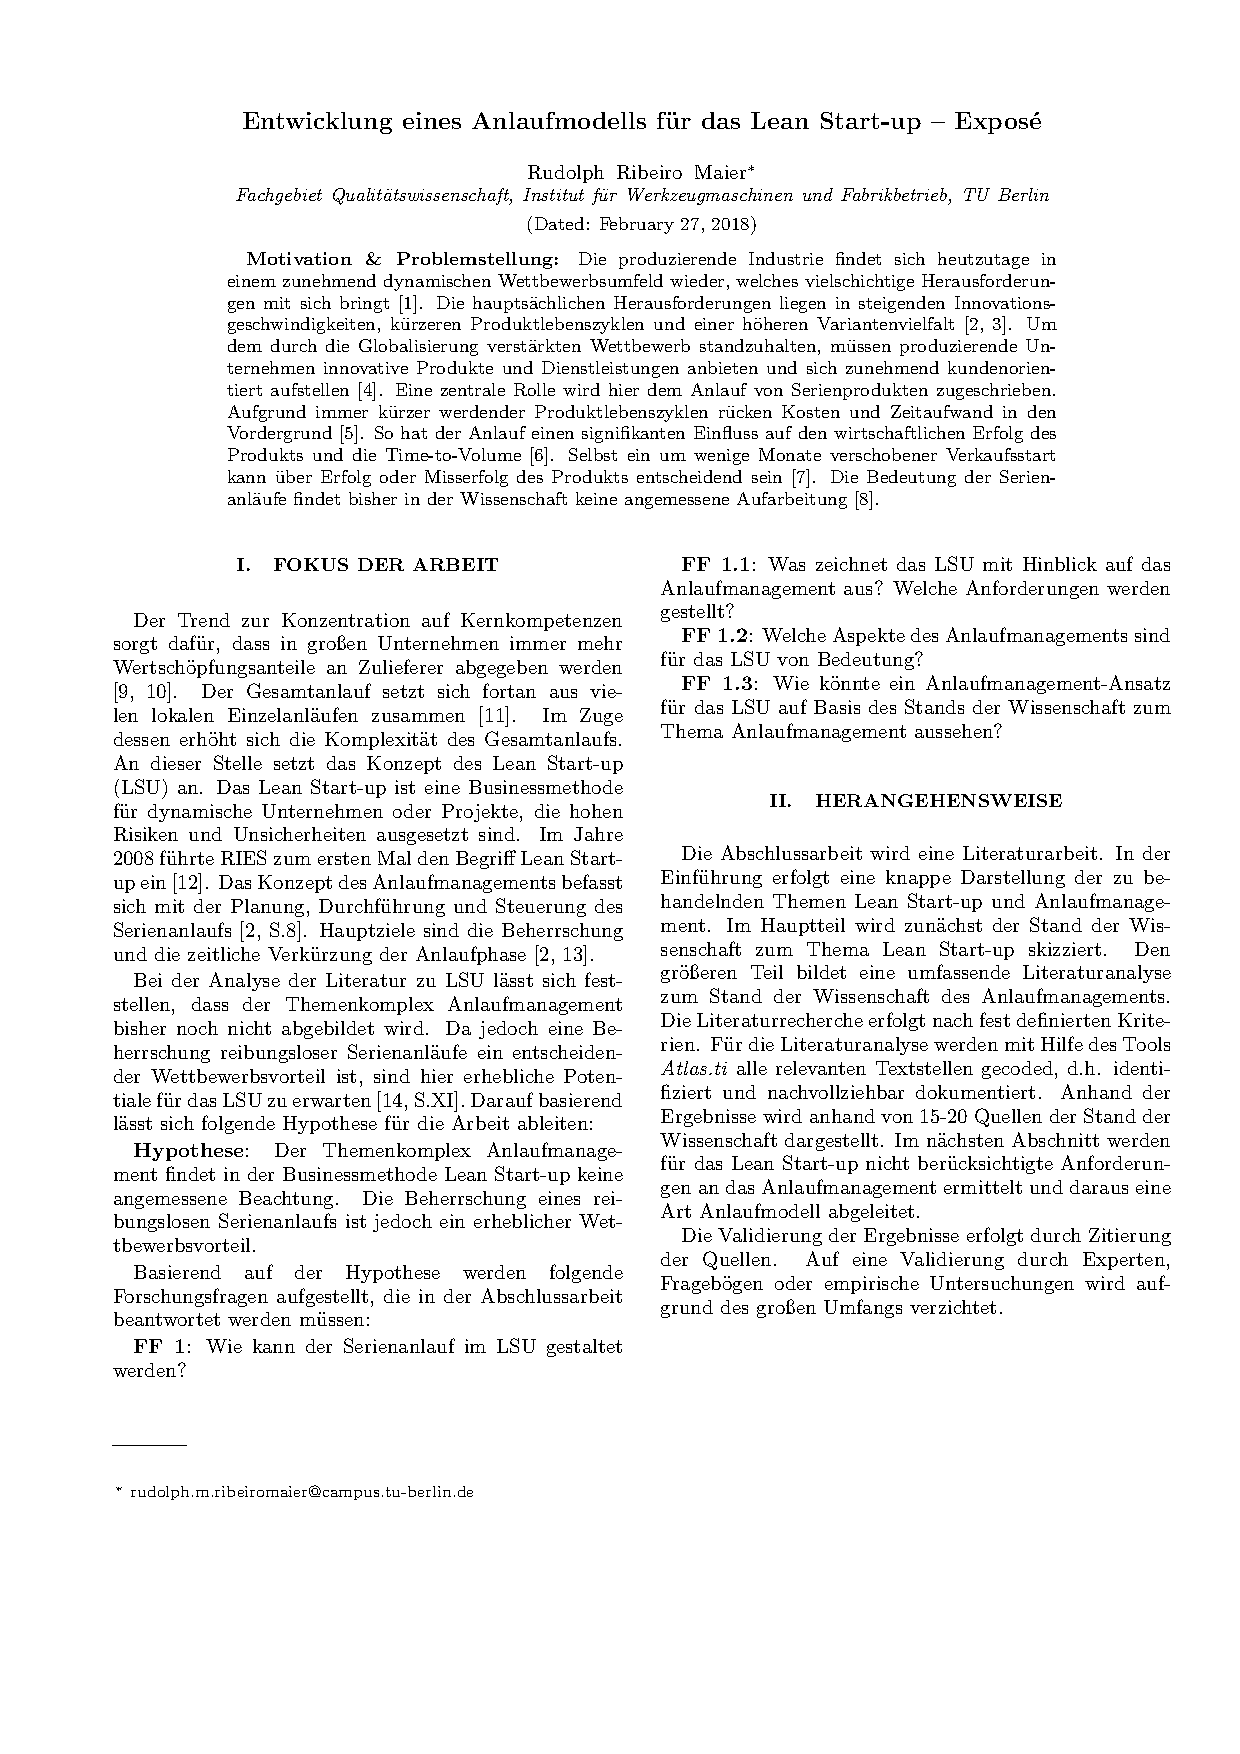
\includepdf[pages={1,2}]{latex_settings/onepager.pdf}			% Aufgabenstellung

% \chapter{Ergänzungen}
\newgeometry{left=30mm, right=30mm, top=20mm, bottom=5mm}
\section{Die Entwicklung des Grundgerüsts}
\begin{figure}[ht]
 \centering
 \includegraphics[scale=.76,clip=true,trim=30 50 30 40]{./img/Kollage.pdf}
 % Kollage.pdf: 0x0 pixel, 300dpi, 0.00x0.00 cm, bb=
 \caption{Entwicklung des Grundgerüsts}
 \label{fig:kollage}
\end{figure}

\clearpage
\restoregeometry

\section{Dombrowski-2011a - Lean Ramp-up. Handlungs- und Gestaltungsfelder}
\subsection*{Die Handlungsfelder im Lean Ramp-up}\label{appendix:dom11a:hf}
\begin{description}

\item[Produktentwicklung und Konstruktion]
umfassen alle Aufgaben, die sich mit
dem Konzipieren, Entwerfen, Ausarbeiten und Erproben eines Produkts
beschäftigen. Als Ergebnis resultieren Zeichnungen, Stücklisten und andere Produktdokumentationen.

\item[Fertigungs- und Montagemittel] umfassen alle Aufgaben, die sich mit der Bedarfsplanung, Auswahl, Beschaffung,
Herstellung, Einrichtung, Programmierung und Inbetriebnahme von Maschinen, Anlagen, Werkzeugen und
Vorrichtungen beschäftigen. Dazu gehören auch die Wartung und Instandhaltung. Als Ergebnis resultiert ein
Fertigungs- und Montagekonzept.

\item[Fertigungs- und Montageprozesse] umfassen alle Aufgaben, die sich mit der
Festlegung der Arbeitsabläufe zur
Herstellung eines Produkts in der
Fertigung und Montage beschäftigen.
Es werden u. a. Reihenfolgen und
Vorgabezeiten bestimmt sowie Produktionsmittel zugeordnet. Als Ergebnis resultieren Arbeitspläne, in
denen alle Informationen dokumentiert sind.

\item[Personal- und Arbeitsorganisation] umfasst alle Aufgaben, die sich mit der
Bedarfs- und Einsatzplanung, Beschaffung, Entwicklung und Freisetzung von Personal sowie mit der Gestaltung einer arbeitsgerechten und
bestmöglichen Zusammenarbeit von
Mensch und Technik beschäftigen.
Als Ergebnis resultieren zum Beispiel
Personaleinsatzpläne,
 Arbeitszeitund Entgeltsysteme.

\item[Produktionsplanung und -steuerung]
(PPS) umfasst alle Aufgaben, die sich
mit der Festlegung, Veranlassung,
Überwachung und Sicherung des Produktionsprogramms nach Art und
Menge unter Berücksichtigung von
Terminen und Kapazitäten beschäftigen. Als Ergebnis resultiert ein Produktionsplan mit Bedarfsmengen und
-terminen für Zukauf- und Eigenfertigungsteile.

 \item[Einkaufs- und Dispositionsprozesse]
umfassen alle Aufgaben, die sich mit
der kostenoptimalen strategischen
und operativen Beschaffung von Zukaufteilen, Handelswaren, Betriebsmitteln und Dienstleistungen von einem Lieferanten beschäftigen. Als Ergebnis resultieren zum Beispiel Sourcingstrategien, Verträge mit Lieferanten und verfügbare Lagerbestände.


 \item[Logistikprozesse und Logistikmittel]
umfassen alle Aufgaben, die sich mit
der Festlegung von effizienten inner-
und außerbetrieblichen Transporten
bzw. Materialflüssen und der Bereitstellung von Gütern beschäftigen.
Außerdem werden Logistikmittel, wie
z. B. Lager- und Transportmittel bestimmt. Als Ergebnis resultieren sog.
Logistiksysteme.

 \item[Gebäude, Layout und Arbeitsplätze]
umfassen alle fabrikplanerischen Aufgaben, die sich mit der Festlegung, optimalen Auslegung und Realisierung
der Produktionsstätten beschäftigen.
Der Umfang reicht dabei von der Umgestaltung einzelner Arbeitsplätze bis
hin zur Errichtung neuer Gebäude.
Als Ergebnis resultieren eingerichtete
Arbeitsplätze, Flächen und Gebäude.


 \item[Qualitätsmanagement und Qualitätsmittel] umfassen alle Aufgaben, die
sich mit der Planung, Lenkung, Prüfung, Sicherung und Verbesserung
der Qualitätsmerkmale von Produkten, Prozessen und Leistungen beschäftigen. Außerdem werden Qualitätsmittel, wie z. B. Prüf- und Messmittel bestimmt. Als Ergebnis resultieren beispielsweise Arbeits- und
Prüfanweisungen.

\item[Informationsprozesse und -systeme]
umfassen alle Aufgaben, die sich mit
der Beschaffung, Verarbeitung, Übertragung und Speicherung von Informationen zur Integration und zielorientierten Steuerung aller operativen Prozesse beschäftigen. Als Ergebnis resultieren zum Beispiel Systeme
zur Betriebsdatenerfassung (BDE).
\end{description}

\subsection*{Die Gestaltungsfelder im Lean Ramp-up}\label{appendix:dom11a:gf}
\begin{description}
\item[Integration und Kooperation] umfassen
alle Methoden und Werkzeuge, die
fachbereichs-, phasen"~, technologie- und unternehmensübergreifend zur
Synchronisierung von Produkt- und
Produktionsentwicklung beitragen.
Dazu wird eine simultane, interdisziplinäre und partnerschaftliche Zusammenarbeit angestrebt. Ziel ist es,
zum Beispiel Schnittstellen und Änderungen zu reduzieren.

\item[Partizipation und Veränderung] umfassen alle Methoden und Werkzeuge,
die zur Motivation der Mitarbeiter
und zum Abbau bzw. zur Vermeidung
von Widerständen und Konflikten beitragen. Dazu werden alle betroffenen
Organisationseinheiten am ProdukBild 4. Gestaltungsfelder im Lean Ramp-up
tionsanlauf beteiligt. Ziel ist es, die
Potenziale der Mitarbeiter zu nutzen
und einen reibungslosen Anlauf zu erreichen.

 \item[Wertschöpfung und Just-in-Time (JIT)]
umfassen alle Methoden und Werkzeuge, die zur produktiven, schnellen
und termingerechten Herstellung
bzw. Lieferung der Produkte beitragen. Dazu werden alle Verluste in den
Produktions- und Logistikprozessen
eliminiert und eine fließende und
kundenorientierte Produktion aufgebaut. Ziel ist ein schlankes Produktionssystem.

 \item[Pilotierung und Qualifizierung] umfasst
alle Methoden und Werkzeuge, die
zur Absicherung von Produkt- und
Prozessreifegrad sowie zur Steigerung der Leistungsfähigkeit des Produktionssystems beitragen. Dazu
werden sog. Pilotbereiche eingerichtet in denen Produktionstests sowie
Mitarbeiterschulungen erfolgen. Ziel
ist eine steile Lern- bzw. Anlaufkurve.

 \item[Priorisierung und Standardisierung]
umfassen alle Methoden und Werkzeuge, die zur Reduzierung, Beherrschung und Vermeidung der technologischen, prozessualen und organisatorischen Komplexität im Produktionsanlauf beitragen. Dazu werden
Schwerpunkte gebildet und Referenzunterlagen erstellt. Ziel ist es, den
Aufwand im Produktionsanlauf zu reduzieren.

 \item[Reaktionsfähigkeit und Flexibilität] umfassen alle Methoden und Werkzeuge,
die zum zeitnahen Erkennen veränderter Randbedingungen und Störungen sowie zur kontinuierlichen Anpassung des Anlaufmanagements beitragen. Dazu werden Frühwarnsysteme etabliert und Handlungsoptionen
bestimmt. Ziel ist es, schnell auf Veränderungen und Störungen zu reagieren.

 \item[Fehler- und Risikovermeidung] umfasst
alle Methoden und Werkzeuge, die
zur präventiven Qualitätssicherung
und -verbesserung beitragen. Dazu
werden frühzeitig die Ergebnisse der
Produkt- und Produktionsentwicklung veranschaulicht und Fehler- bzw.
Risikopotentiale eliminiert. Ziel sind
eine hohe Produkt- und Prozessqualität sowie geringe Änderungs- und
Prüfkosten.

 \item[Problemlösung und Stabilisierung] umfassen alle Methoden und Werkzeuge,
die zur reaktiven Qualitätssicherung
und -verbesserung beitragen. Dazu
werden die Produkte und Prozesse
kontinuierlich überprüft und überwacht sowie systematisch Problemursachen beseitigt. Ziel ist eine Stabilisierung des Anlaufs und Vermeidung
von Folge- und Wiederholungsfehlern.

 \item[Wissenstransfer und KVP] umfassen
alle Methoden und Werkzeuge, die
zum Transfer von Erfahrungswissen
und zur Erhöhung der Mitarbeiterkompetenzen beitragen. Dazu wird
explizites und – soweit möglich – implizites Wissen identifiziert, gesammelt, aufbereitet und vermittelt. Ziel
ist es, mit dessen Nutzung und
Weiterentwicklung aktuelle und zukünftige Anläufe zu verbessern.

 \item[Transparenz und Visualisierung] umfassen alle Methoden und Werkzeuge,
die zur Verfügbarkeit und leicht verständlichen Darstellung von Informationen und Daten beitragen. Dazu
werden sowohl informations- und
kommunikationstechnische Systeme
als auch optische Hilfsmittel und Signale eingesetzt. Ziel ist die Regelung,
Steuerung und Verbesserung des Produktionsanlaufs.
\end{description}


\newpage
%   left=30mm, right=30mm, top=20mm, bottom=20mm, % margins

\newgeometry{left=30mm, right=30mm, top=20mm, bottom=5mm}
\section{Dombrowski-2011b - Lean Ramp-up: Schwerpunkte im Anlaufmanagement}
\begin{figure}[h!]
 \centering
 \includegraphics[scale=.3]{./img/dom11b:firstmover.png}
 % dom11b:firstmover.png: 0x0 pixel, 0dpi, 0.00x0.00 cm, bb=
 \caption[Schwerpunkte für \textit{Firstmover}]{Schwerpunkte für \textit{Firstmover} \autocite{Dombrowski2011b}}
 \label{fig:dom11b:firstmover}
 \vspace{8mm}
% \end{figure}
% 
% 
% \begin{figure}[h]
 \centering
 \includegraphics[scale=.3]{./img/dom11b:kostenfuehrer.png}
 % dom11b:firstmover.png: 0x0 pixel, 0dpi, 0.00x0.00 cm, bb=
 \caption[Schwerpunkte für \textit{Follower (Kosten)}]{Schwerpunkte für \textit{Follower (Kosten)} \autocite{Dombrowski2011b}}
 \label{fig:dom11b:kostenfuehrer}
 \vspace{8mm}
% \end{figure}
% 
% 
% \begin{figure}[h]
 \centering
 \includegraphics[scale=.3]{./img/dom11b:qualitaetsfuehrer.png}
 % dom11b:firstmover.png: 0x0 pixel, 0dpi, 0.00x0.00 cm, bb=
 \caption[Schwerpunkte für \textit{Follower (Qualität)}]{Schwerpunkte für \textit{Follower (Qualität)} \autocite{Dombrowski2011b}}
 \label{fig:dom11b:qualitaetsfuehrer}
%  \vspace{5mm}
\end{figure}
\restoregeometry  
\newpage
\blankpage
\end{document}
